\section{Utilisation du logiciel}

La figure suivante montre l'interface utilisateur du logiciel.

{\centering 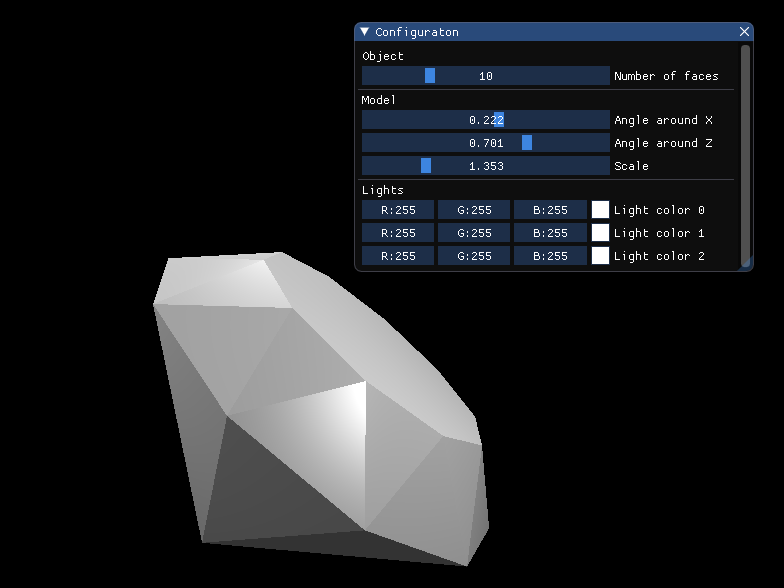
\includegraphics[width=0.8\textwidth]{screenshot_software_2}}

Il est possible de déplacer la caméra à l'aide des touches WASD sur un clavier qwerty ou ZQSD sur un clavier azerty
(le mappage est physique et ne dépend donc pas de la disposition du clavier).
La touche espace permet de faire s'élever la caméra tandis que la touche contrôle permet l'abaisser.

\begin{wrapfigure}{r}{0.51\textwidth}
    \centering
    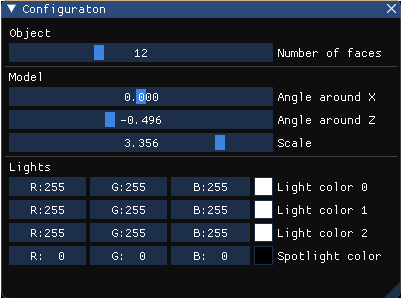
\includegraphics[width=0.5\textwidth]{config_window}
\end{wrapfigure}
Une fenêtre de configuration flottante permet de configurer la scène.
Comme on peut le voir sur la figure, il est possible de configurer le nombre de
faces inférieures du diamant, de changer son orientation et sa taille, mais aussi
de configurer les lumières.
Il est possible «~d'éteindre~» les lampes en réglant leur couleur sur noir.
Par défaut, la torche accrochée à la caméra est éteinte.

Lorsque le curseur n'est pas sur la fenêtre de configuration, cliquer et déplacer la souris permet
d'orienter la caméra.

